\section{Analyse von Funktion F220: Ausleihe}
\label{f:220}
Ein oder mehrere Dokumente werden von einem Benutzer ausgeliehen. Dabei wählt 
der Benutzer das gewünschte Dokument aus und das System muss in der Datenbank 
nachprüfen, ob dieses derzeit ausleihbar ist. Wenn dies der Fall sein sollte, 
wird dem Benutzer dieses Buch zugewiesen. Dies erfolgt durch zwei 
Built-In-Funktionen von \gls{glos:django}, mit dessen Hilfe die Datenbank 
erweitert bzw.\ ein Datensatz geupdatet werden kann. Es gehört zum 
\textbf{View}-Komponent im Zusammenhang zur \textbf{DB}.

\begin{figure}[H]
\begin{center}
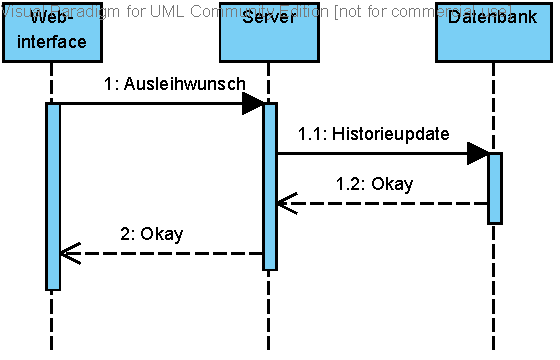
\includegraphics[width=0.6\linewidth]{bilder/seq-uebertragen.pdf}
\caption{Sequenzdiagramm für eine Ausleihe}
\label{fig:220}
\end{center}
\end{figure}

Das Sequenzdiagramm verdeutlicht nochmal, dass erst der Ausleihwunsch an den Server übermittelt wird. Dieser wandelt diesen Wunsch dann für die Datenbank verständlich um, wodurch dort die Datensätze geupdatet werden. Darauf folgt ein Okay an den Server der diesen ans Web-Interface weitergibt.

\section{Analyse von Funktion F221: Ausleihe an Externe}
\label{f:221}
Die Ausleihe an \gls{glos:ext} ist ähnlich gestaltet wie in \ref{f:220} 
\nameref{f:220} und gehört ebenfalls dem \textbf{View}-Komponent mit 
\textbf{DB}-Einflüssen. Es existiert lediglich der Zusatz, dass der Benutzer 
einen \gls{glos:ext}n als eigentlichen Ausleiher angibt. Dafür wird beim 
Entleihen die Möglichkeit gegeben, Daten über den \gls{glos:ext}n anzugeben, 
dessen Daten dann gespeichert und beim Entleihen vermerkt werden. Auch hierbei 
wird eine Built-In-Funktion zum Erweitern der Datenbank genutzt.

\begin{figure}[H]
\begin{center}
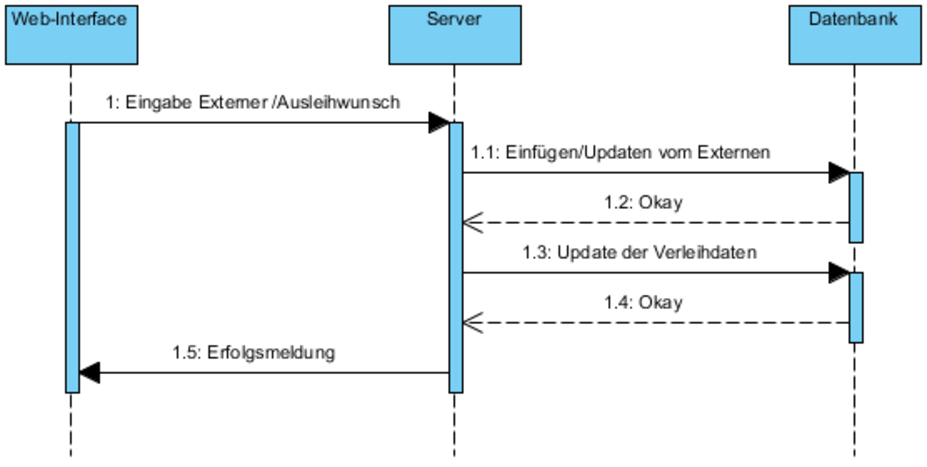
\includegraphics[width=0.8\linewidth]{bilder/Seq-Ausleihe.pdf}
\caption{Sequenzdiagramm für Ausleihe an Externe}
\label{fig:221}
\end{center}
\end{figure}
Wie das Sequenzdiagramm aufzeigt, wird zuerst die ein Ausleihwunsch mit Eingabe eines Externen getätigt. Diese Daten gelangen an den Server, der zuerst den Externen in die Datenbank einträgt und dann die Verleihdaten aktualisiert. Sollte alles so abgelaufen sein wie es gewollt ist, bekommt der Server ein Okay zurück und gibt dieses weiter ans Web-Interface.

\section{Analyse von Funktion F222: Ausleihe übertragen}
\label{f:222}
Ein Dokument wechselt den Ausleihenden. Dabei muss ein Benutzer $A$ ein von ihm 
ausgeliehenes Dokument auswählen und einem anderen Benutzer $B$ übertragen. 
Alternativ kann Benutzer $B$ auch eintragen, dass er sich ein Dokument von 
Benutzer $A$ geholt hat, das Dokument also jetzt bei ihm zu finden ist. Das 
System vermerkt dieses Austausch dann in der Datenbank mittels einer 
Built-In-Funktion von \gls{glos:django}. Auch diese gehört zur 
\textbf{View}-Komponente mit Zugriff auf die \textbf{DB}.

\begin{figure}[H]
\begin{center}
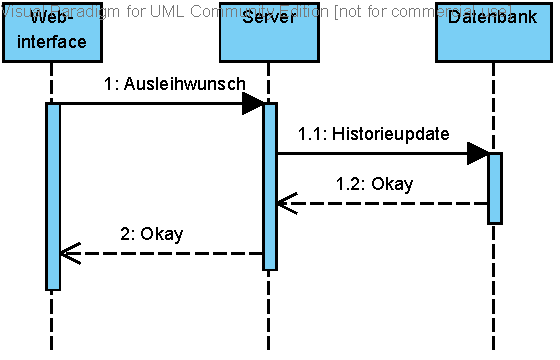
\includegraphics[width=0.6\linewidth]{bilder/seq-uebertragen.pdf}
\caption{Sequenzdiagramm für eine Ausleihe übertragen}
\label{fig:222}
\end{center}
\end{figure}
Auch hier verdeutlich das Sequenzdiagramm, dass nur ein Ausleihwunsch an den Server übermittelt wird, worauf dieser, nach einer Historieupdate-Anweisung an die Datenbank, ein Okay von dieser zurückbekommen sollte und das Okay sofort an das Web-Interface weitergibt.

\section{Analyse von Funktion F223: Ausleihe zurückgeben}
\label{f:223}
Ein Benutzer braucht ein Dokument nicht mehr und gibt es in den Bestand der 
Bibliothek zurück. Auch hierfür muss der Benutzer als Entleiher des Dokumentes 
eingetragen sein. Wenn dies der Fall sein sollte, kann er \emph{zurückgeben} 
wählen und das Dokument wird auch im Datensatz mittels Built-In-Funktionen von 
\gls{glos:django} mit dem Status 0 versehen. Die Funktion ist dem \textbf{View} 
zugeordnet, benötigt aber auch die \textbf{DB}.

\begin{figure}[H]
\begin{center}
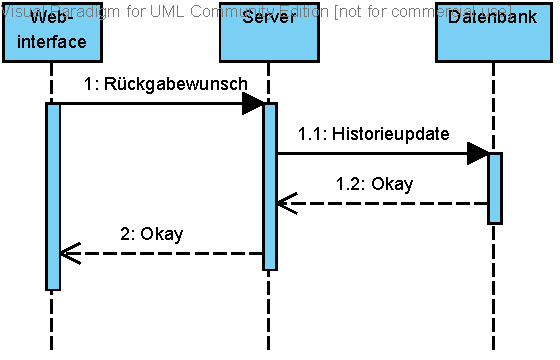
\includegraphics[width=0.6\linewidth]{bilder/seq-zurueck.pdf}
\caption{Sequenzdiagramm für eine Ausliehe zurückgeben}
\label{fig:223}
\end{center}
\end{figure}
Wie im Sequenzdiagramm zu sehen, wird zuallererst einmal ein Rückgabewunsch an den Server getätigt. Der gibt die entsprechenden Anweisungen an die Datenbank weiter. Daraufhin erfolgt ein Okay von der Datenbank an den Server und von dort aus ans Web-Interface.

\section{Analyse von Funktion F224: Ausleihe vermisst melden}
\label{f:224}
Das Dokument befindet sich nicht mehr an dem laut Datenbank befindlichen Ort. 
Dann kann ein Benutzer ein Dokument auf der Dokumentenansicht als 
\emph{vermisst} melden und dieses wird in der Datenbank mittels Statusänderung 
vermerkt. Dazu wird eine E-Mail an alle Benutzer verschickt oder alternativ eine
Meldung auf der Homepage angezeigt. Hierfür stellt \gls{glos:django} wieder 
Built-In-Funktionen bereit. Das Ganze gehört dann zu \textbf{View} und 
\textbf{DB}.

\begin{figure}[H]
\begin{center}
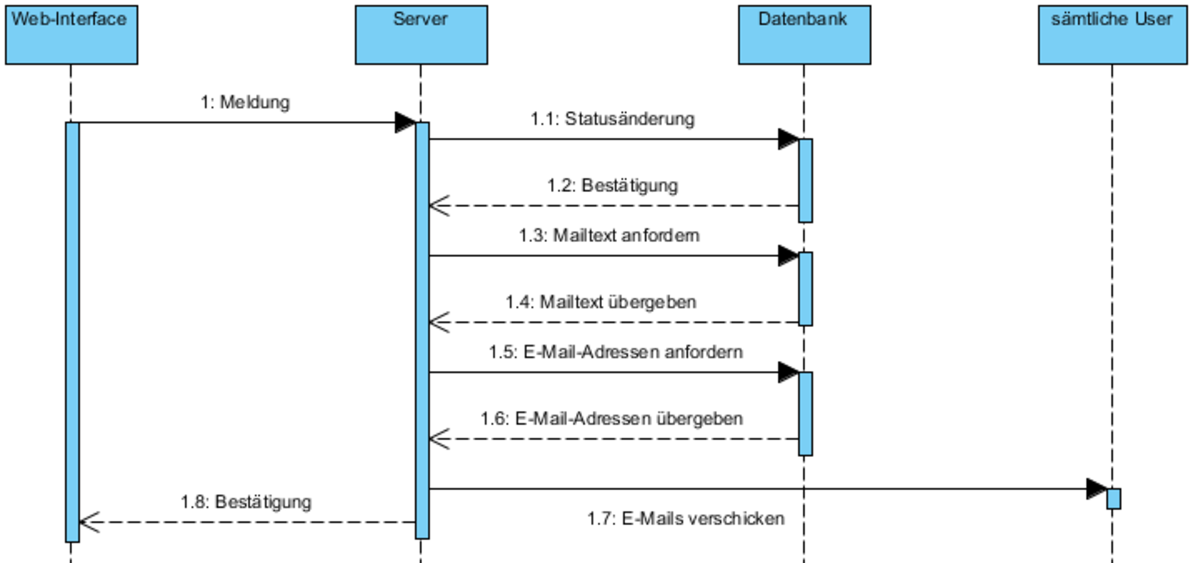
\includegraphics[width=0.9\linewidth]{bilder/Seq-Vermisst.pdf}
\caption{Sequenzdiagramm für eine Vermisstmeldung}
\label{fig:224}
\end{center}
\end{figure}
Diesmal beginnt das Ganze mit einer Meldung an den Server. Dieser lässt die Datenbank den Status des Dokumentes ändern und sollte darauf eine Bestätigung erhalten. Danach werden Mailtext und E-Mail-Adressen angefordert, welche die Datenbank beide an den Server ausgeben müsste. Daraufhin bekommen sämtliche User eine E-Mail vom Server zugeschickt und ans Web-Interface geht eine Bestätigung.

\section{Analyse von Funktion F225: Ausleihe verloren melden}
\label{f:225}
Das Dokument ist auch nach einer Vermisstenmeldung nicht wieder aufgetaucht. 
Dann ist ein Bibliothekar berechtigt, es als \emph{verloren gegangen} 
einzustufen. Das Dokument bekommt den entsprechenden Status und wird demnächst 
bei weiteren Suchanfragen ausgeschlossen. Dies erfolgt wieder innerhalb der 
\textbf{View}- und \textbf{DB}-Komponenten durch eine Built-In-Funktion von 
\gls{glos:django}.

\begin{figure}[H]
\begin{center}
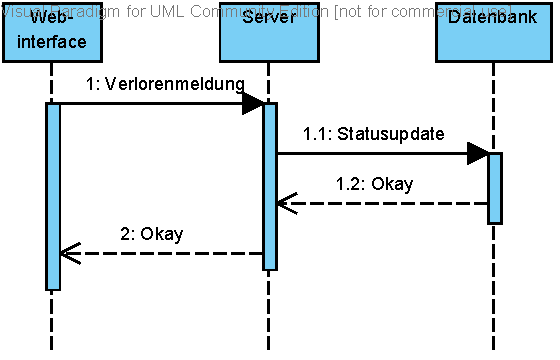
\includegraphics[width=0.6\linewidth]{bilder/seq-verloren.pdf}
\caption{Sequenzdiagramm für eine Verlorenmeldung}
\label{fig:225}
\end{center}
\end{figure}
Auch hier beginnt alles mit einer Meldung an den Server. Jedoch wird darauf nur ein Statusänderungsauftrag an die Datenbank weiter gegeben und schon erfolgt ein Okay an den Server, der diesen ans Web-Interface weiterreicht.
